\documentclass{ctexart}
\usepackage{graphicx}

\author{[REMOVED]<[REMOVED]>\\学号:[REMOVED]}
\title{微机原理实验2\\汇编语言编写Fibonacci数列}
\begin{document}

\begin{titlepage}
\maketitle
\thispagestyle{empty}
\newpage
\tableofcontents
\thispagestyle{empty}
\end{titlepage}

\setcounter{page}{1}

\section{题目简介} 

使用ARM汇编语言编写程序,计算出Fibonacci数列的前30项,并在Keil C中仿真。Fibonacci数列的一个定义是:
\[\{F_n\}_{n=0}^\infty\]
并定义\(F_{0}=0\),\(F_{1}=1\),且
\[F_{n}=F_{n-1}+F_{n-2}\]
。

\section{题目分析}

\subsection{介绍}
由于本题不允许使用C语言嵌入汇编,因此需要处理的比较多。

首先要处理的是栈指针和中断向量。按照内核设计,启动后ROM会被映射到0x80000000开始的512KBytes中,且内核会读取第一个值作为sp的初值,之后读取的值作为中断向量。由于Cortex-M3的模拟内核功能不多,只模拟了复位中断(即Reset\_Handler),因此我们的程序只要在前部写好中断向量的地址就好了。为了简化代码,中断向量可以直接接入一段跳转代码,跳转入我们的主程序中。

之后就可以写主程序了。主程序设计比较简单,为了提高速度,没有做空间优化,使用了六个寄存器。其中$R0$作为循环终值,$R1$代表要存放结果的空间。程序运行后,会把数列的\(F_{0},F_{1},\cdots,F_{R0}\)项存储入$R1$开始的地址空间中,所有的值均为无符号整型。$R4$、$R5$分别用于储存数列的第\(F_{n-2}\)、\(F_{n-1}\)项,$R6$用于保存当前循环值n,$R7$则用来保存计算得到的\(F_{n}\)。

\subsection{程序分析}

按照以上思路编写的程序如下:

\begin{center}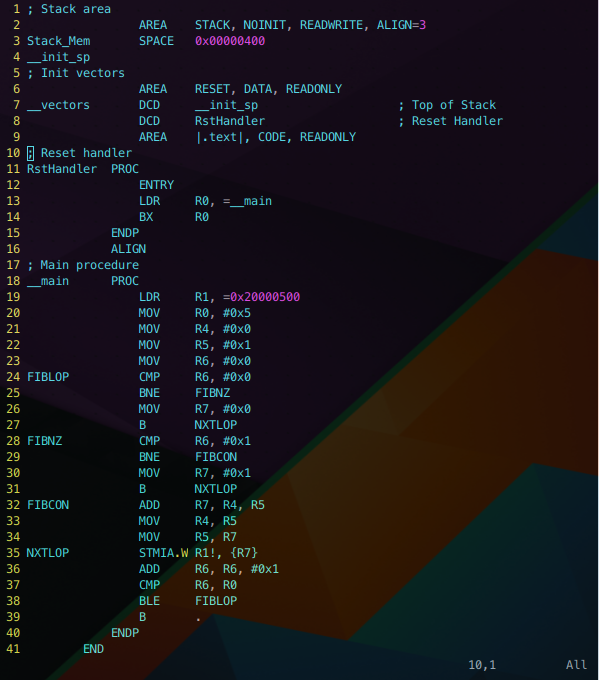
\includegraphics[width=11cm]{./img/code.png}\end{center}

首先关注前4行,这里在一块可写区域(链接器会理解为SRAM区段)申请了0x400字节长度的内存,并加标号\_\_init\_sp。

从第5行开始,所有的代码都会被链接器放在EEPROM对应的区段。5~8行声明了SP的初值(第7行)和复位中断对应的向量(第8行)。

从第11行开始,是中断向量的处理子程序,其中12行额外将这个子程序作为入口点。13行和14行导入了主程序对应的值,并跳转到主程序。

19~23行处理了主程序需要的参数,并填入了初始化值。24~27、28~31、32~34分别对应了$n=0$、$n=1$和$n>1$时的运算,35行将参数存入对应地址中并自增地址,之后进入下一次循环,直到循环打到预计的终值。

\subsection{程序调试}

下面是调试过程中几个关键点的截图,分别截取在$R6=0,1,5,29$时。

\begin{center}
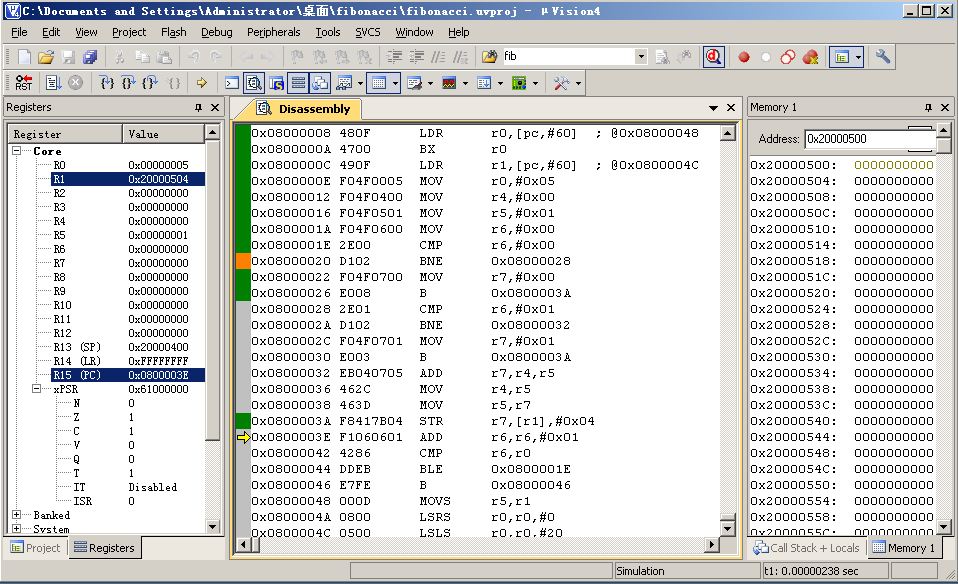
\includegraphics[width=11cm]{./img/debugzero.png}
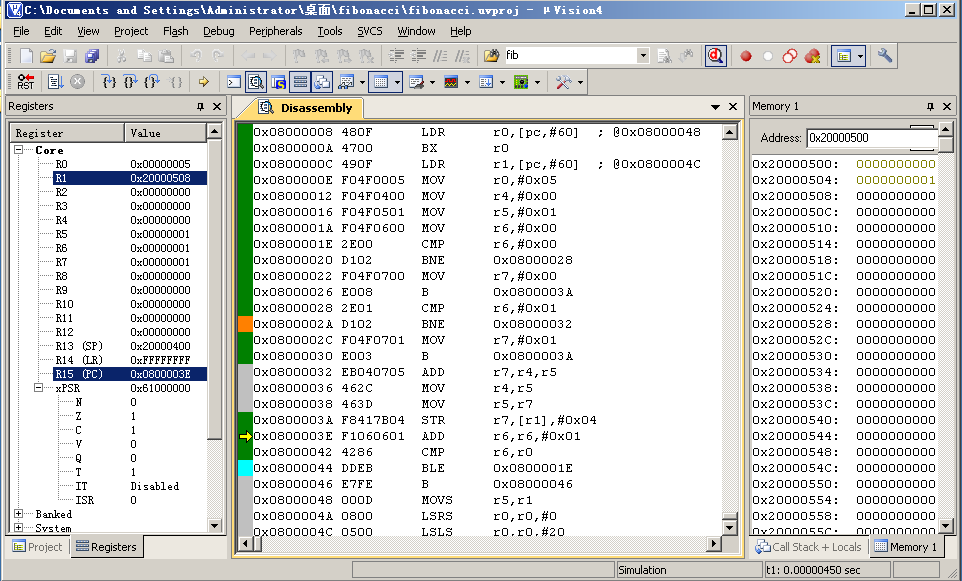
\includegraphics[width=11cm]{./img/debugone.png}
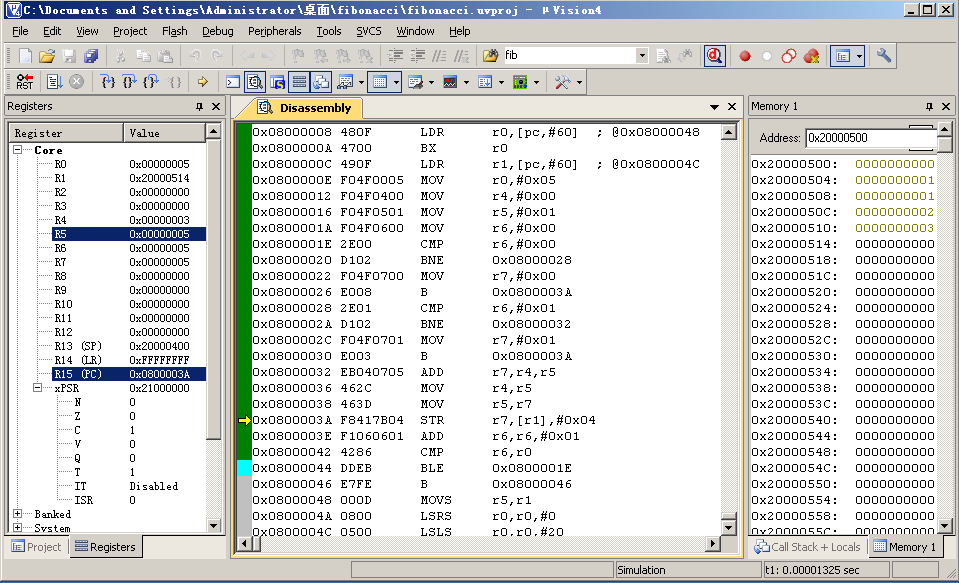
\includegraphics[width=11cm]{./img/debugfive.png}
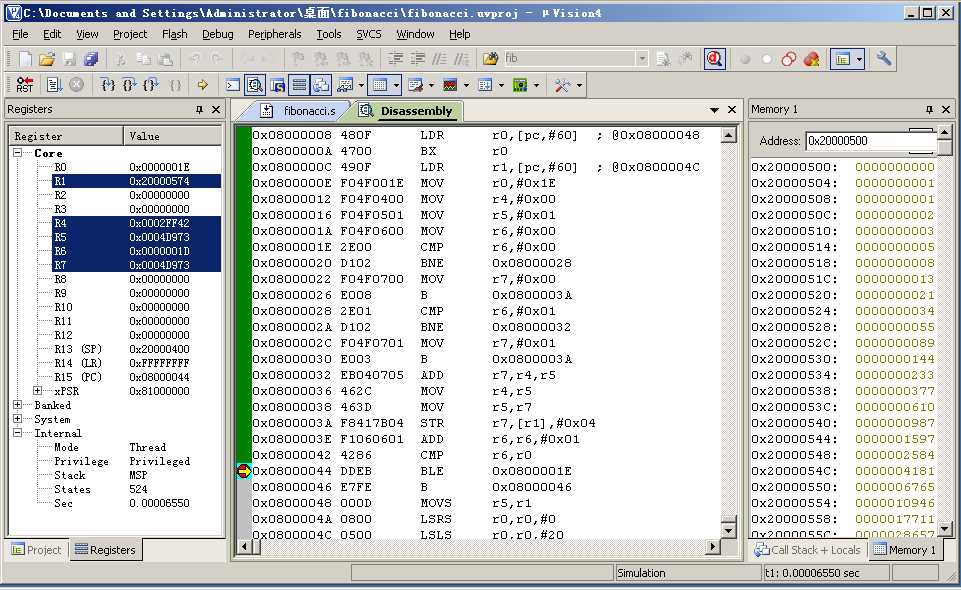
\includegraphics[width=11cm]{./img/debugall.png}
\end{center}

\section{附件列表}

fibonacci.s: 源代码\\
fibonacci.uvproj: 工程文件\\
fibonacci.sct: 链接控制文件\\
asm\_fibonacci.tex: 本文源码等\\
asm\_fibonacci.pdf: 本文文件

\end{document}
